\chapter{Métodos}

A todas as experiências foram aplicadas as métricas apresentadas, excepto no benchmark onde teríamos métricas de comparação a ele próprio.\\
Para a escolha de melhor modelo dentro das experiências foi escolhido o modelo que melhor resultados apresentou para a métrica em questão. Sendo esta o GPD $Norm^{2}$ enquanto não encontramos uma melhoria tanto na alocação em falta como na em demasia, ao que se seguida foi usado o GPD Positivo.\\
No caso das Redes Neuronais a hiper parametrização foi feita também deste modo, sendo que primeiro se encontrou uma hiper parametrização adequada aos dados, usando uma arquitetura simples e só depois com essa configuração foi feita a experiência  nas várias arquiteturas.\\
O objectivo é conseguir um modelo que tenha a uma Alocação Total em Falta e Alocação Total em Demasia menor que o Benchmark, dentro dos anos 2019 a 2022. Logo em termos de métricas um GPD Positivo mais elevado possível.\\

\thispagestyle{plain}
\section{Estatisticos}

Em estatística conseguimos encontrar vários métodos de estudo de séries temporais. Estes métodos são normalmente usados como primeira abordagem para fazer previsões.\\
Estes modelos podem ser auto-regressivos (AR), onde vão fazer previsões baseados num número (p) de dados anteriores. Estes modelos são construídos com a noção de que um valor é linearmente dependente de p valores anteriores numa série temporal.\\

\begin{alignat*}{2} 
    & X_{t} : \text{Valor no } t \text{ a prever.} &\quad& p : \text{O número observaçoes anteriores.} \\
    & \varphi_{i} : \text{Coeficiente na observação } i. &\quad& q : \text{O número observaçoes anteriores.} \\
    & \epsilon_{i} : \text{Erro na observação } i. &\quad& \theta_{i} : \text{Coeficiente na observação } i \text{.} \\ 
    & \mu : \text{Média dos valores } X \text{.} 
\end{alignat*}

\bigskip
AR - Auto-Regressivos \\

\begin{equation} \label{eq:ar} 
    X_{t} = \sum_{i=1}^{p}\varphi_{i} X_{t-i} 
\end{equation}
\smallskip

Outra família destes modelos são os de média móvel (MA), onde a média de um número de observações (q) em conjunto com os erros ($\epsilon$) e os coeficientes ($\theta$) é usada para prever os valores seguintes.\\
\bigskip
MA - Média Móvel \\

\begin{equation} \label{eq:ma} 
    X_{t} = \mu + \sum_{i=1}^{q}(\theta_{i} \epsilon_{t-i}) + \epsilon_{t}
\end{equation}
\smallskip
Estes dois tipos de modelos podem ser juntos criando os modelos auto-regressivos de média móvel (ARMA). que junta as capacidades dos modelos anteriores.\\

\bigskip
MA - Média Móvel \\

\begin{equation} \label{eq:ma} 
    X_{t} = \sum_{i=1}^{p}\varphi_{i} X_{t-i}  + \mu + \sum_{i=1}^{q}(\theta_{i} \epsilon_{t-i}) + \epsilon_{t}
\end{equation}
\smallskip

Existem mais modelos de previsão estatística baseados nestes com algumas variações, mas para este trabalho, e apenas como ponto de comparação às redes neuronais, ficamos apenas por estes.\\
As variáveis em estudo por tipo de modelo foram retiradas das autocorrelações temporais usando os métodos de sugestão da ferramenta \hyperref[se:muaddib]{MuadDib}:\\


\begin{table}[h] \centering
\begin{tabular}{lrrrr}
    \toprule
     & p & q \\
    \midrule
    AR & 1/ 2 / 23 / 24 / 25 / 48 / 144 / 168 / 192 / 336 & NA \\
    MA & NA & 1 / 24 \\
    ARMA & 1 & 1 \\
    \bottomrule
    \end{tabular}
    \label{tab:varsstats} 
    \caption{Variáveis de estudo dos modelos AR/MA}
\end{table}


Todos estes modelos foram testados usando o software disponível na package de python \href{https://www.statsmodels.org/stable/index.html}{statsmodel}, com a classe \href{https://www.statsmodels.org/stable/generated/statsmodels.tsa.arima.model.ARIMA.html}{ARIMA}.
 \label{se:metstats}


\newpage
\thispagestyle{plain}
\section{Redes Neuronais}
 \label{se:metneuralnet}

\thispagestyle{plain}
\section{Dados de Validação}
Os dados de validação são os mesmos que os dados de treino, embora apenas durante os anos de 2019 a 2022, inclusive.\\
Usamos como benchmark as capacidades alocadas, "SecondaryReserveAllocationAUpward" e "SecondaryReserveAllocationADownward", e como validação e objectivo, \hyperref[se:metneuralnet]{y}, a própria energia usada, "UpwardUsedSecondaryReserveEnergy" e "DownwardUsedSecondaryReserveEnergy".

\section{Benchmark}

Como método de comparação a todas as experiências foi criado uma base que servirá de benchmark.\\
Este base não é nada mais do que a própria previsão feita pela entidade reguladora ESIOS. Dentro do nossos dados são os valores nos campos "SecondaryReserveAllocationAUpward" e "SecondaryReserveAllocationADownward".\\
Para os dados utilizados, podemos ver a totalidade e comparação do benchmark (Energia Alocada) com a energia utilizada.\\

\begin{figure}[H]
    \centering
    \includegraphics[width=\textwidth]{plots/alocacoes_originais.png}
    \caption{Série Temporal dos dados de Benchmark c/ consumo real}
    \label{fig:benchmarktimeseries}
\end{figure}

Imediatamente podemos verificar que o método para prever a energia necessária actualmente está dentro de um espectro limitado de valores, sendo que esses valores estão perto dos valores de ponta na alocação para cima, e perto dos valores médios na alocação para baixo.\\
Isto deve-se ao facto de ser uma função fixa, baseado no dia em questão. Notamos também que a meio de 2022 houve uma mudança dessa função que limitou os alcances tornando os valores mais elevados. Devido à guerra na Ucrânia e à forte incerteza que esta trouxe aos mercados de eletricidade por causa da crise de gás na Europa, que aumentou significativamente o preço deste recurso e levou à adaptação dos consumidores e países, a Red Eléctrica de España (REE) aumentou as necessidades de reserva secundária para responder a esta incerteza.\\
Do ponto de visto de dados faz sentido para diminuir a quantidade  de vezes em que não é alocada energia suficiente.\\
Mas o mais importante a notar é a forma estática destes métodos, dado a natureza flutuante dos da energia necessária este método apresenta frequentemente um erro grande.\\
Podemos ver em pormenor analisando algumas janelas temporais dentro do período de validação. Vendo o melhor e pior resultado, em termos de erro absoluto, em janelas temporais de ano, mês, semana e dia.\\


\begin{figure}[H]
    \centering
    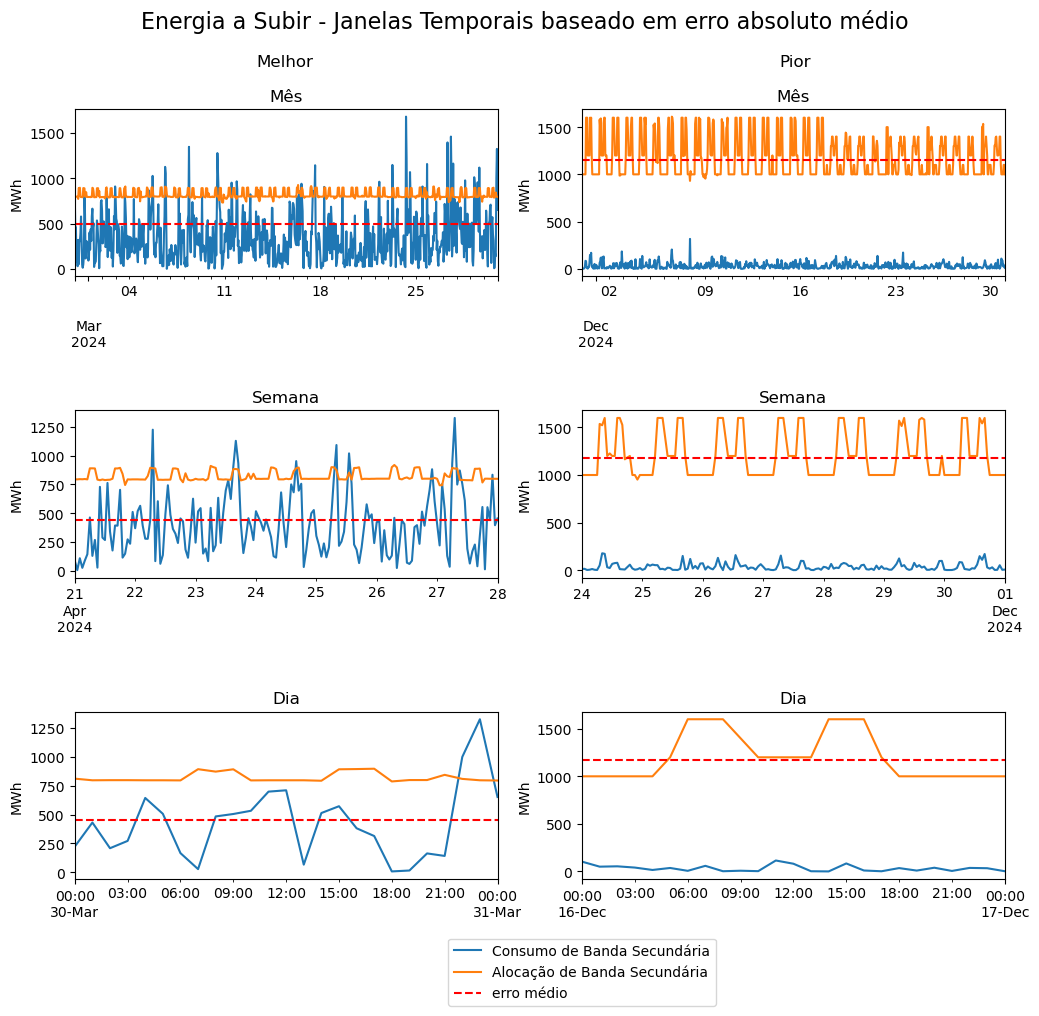
\includegraphics[width=\textwidth]{plots/alocacoes_temporais_upward_dataset.png}
    \caption{Janelas temporais de benchmark energia a subir}
    \label{fig:benchmarktimewindowsup}
\end{figure}


\begin{figure}[H]
    \centering
    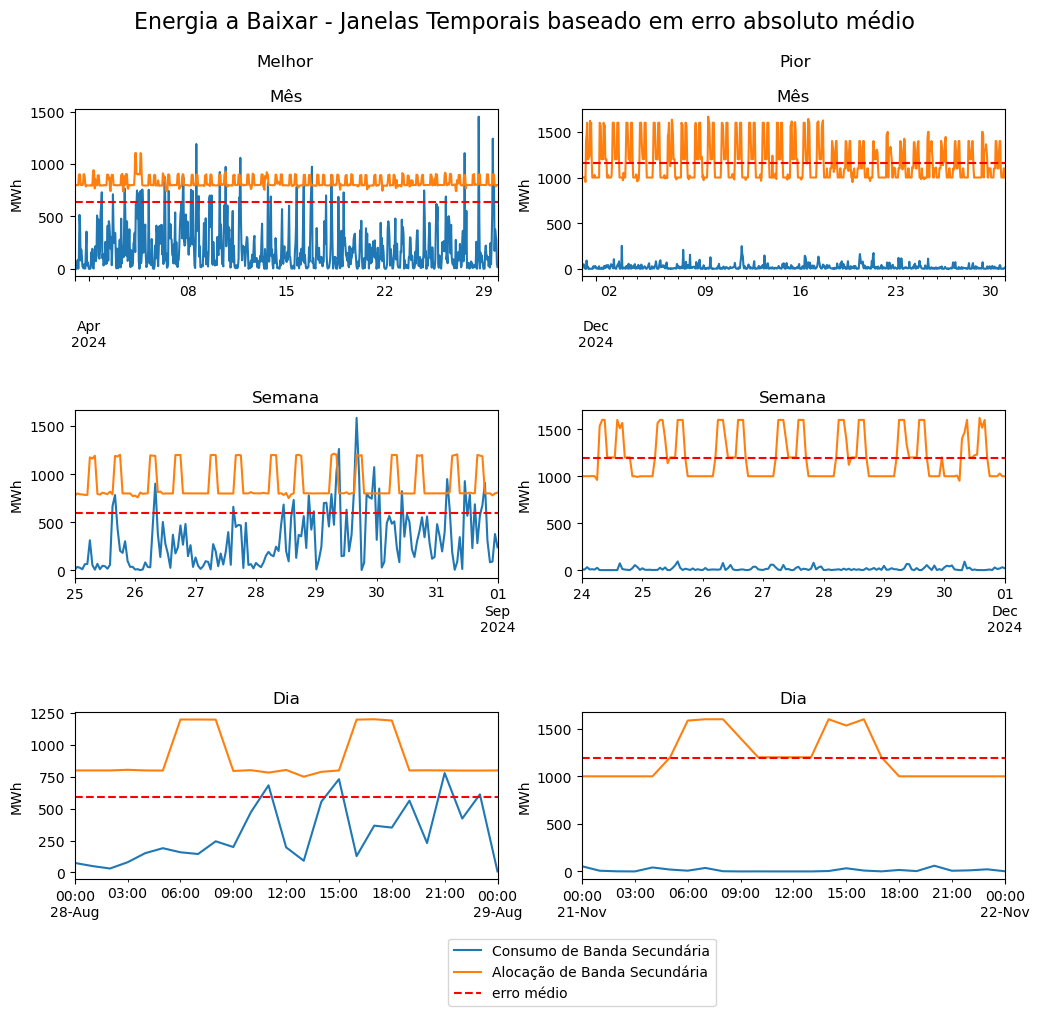
\includegraphics[width=\textwidth]{plots/alocacoes_temporais_downward_dataset.png}
    \caption{Janelas temporais de benchmark energia a descer}
    \label{fig:benchmarktimewindowsdown}
\end{figure}

Dentro destas janelas temporais conseguimos ter melhor a percepção da natureza estática deste modelo actual, e qual longe está dos valores reais necessários.\\





% Neste capitulo percorremos as experiências realizadas. Estas foram feitas atraves do usos do programas criados para o efeito, disponiveis no repositorio GitHub do \href{https://github.com/JotaFan/renewable-generation-into-reserve-markets}{projecto}.\\

% \section{Benchmark}

% Como modelo benchmark iremos usar a alocação feita. Pois são estes valores que procuramos melhorar no caso prático.\\



% \begin{figure}[H]
%     \centering
%     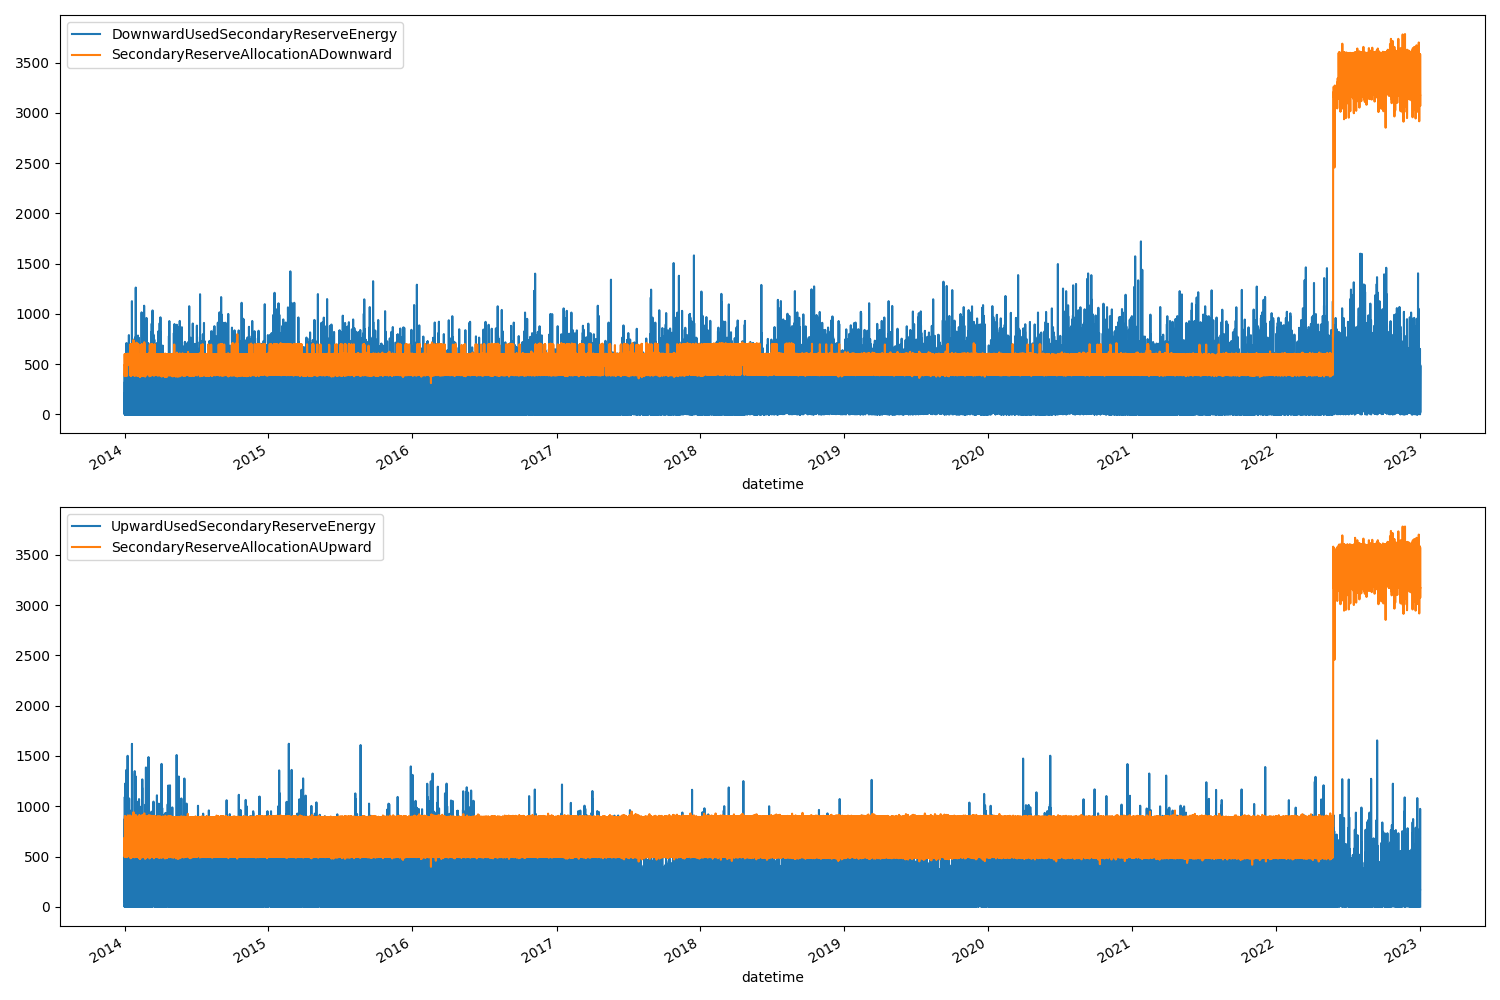
\includegraphics[width=0.8\textwidth]{plots/benchmark.png}
%     \caption{Serie Temporal do benchmark}
%     \label{fig:benchmark}
% \end{figure}
  

% \begin{table}[H]
%     \caption{Dados Benchmark}
%     \resizebox{\linewidth}{!}{\csvautotabular{../data/benchmark_scores.csv}\label{tb:benchmark}}       
% \end{table}


% Para validação dos mesmo, vamos usar o ano 2021, devido aquele salto nos valores de alocação em 2022.\\

% Para esses temos os seguintes dados:

% \begin{figure}[H]
%     \centering
%     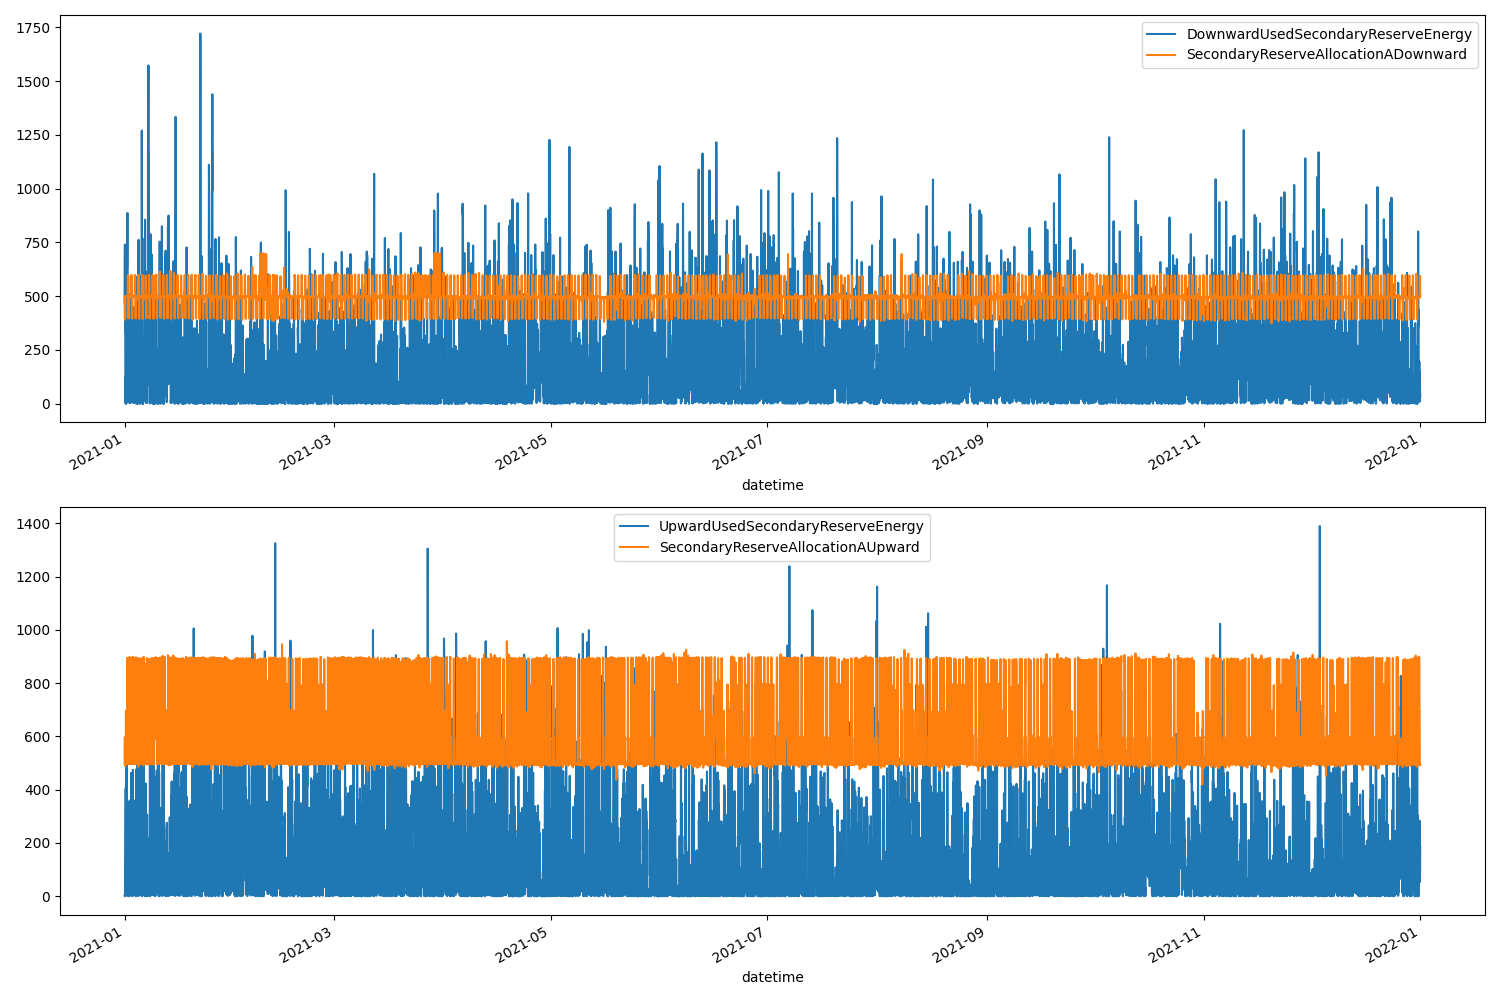
\includegraphics[width=0.8\textwidth]{plots/benchmark_validation.png}
%     \caption{Serie Temporal do benchmark 2021}
%     \label{fig:benchmark_validation}
% \end{figure}
  

% Os metodos em estudo vão ser comparados a esta medida. Sendo que o principal é baixar tanto a alocação perdida, como a alocação a mais. Que se traduzem no erro absoluto.\\

% \begin{table}[H]
%     \caption{Dados Benchmark de validação}
%     \resizebox{\linewidth}{!}{\csvautotabular{../data/benchmark_validation_scores.csv}  \label{tb:benchmark_val}}      
% \end{table}

% \section{Modelos estatiscos\label{se:model_stats}}

% Antes de entrar para o densenvolvimento de modelos vamos usar metódos e modelos abertos para usar comparativamente.\\

% Os modelos estatiscos recurrentes em previsões são AR, MA, ARMA, ARIMA, SARIMA para previsões so com um atributo, e para multiplos atributos VAR.\\
% O modelo AR e o VAR não obtiveram resultados aplicaveis, logo foram desconsiderado.\\

% \subsection{Univariate Analysis}

% Estas análises apenas aplicam uma formula à variavel em questão.

% \subsubsection{AR}
% \begin{equation} \label{eq:AR} 
%     y_t = \beta_0 + \beta_1 y_{t-1} + \dots + \beta_p y_{t-p} + \epsilon_t 
% \end{equation}
% onde:
% \begin{itemize}
%   \item $y_t$: O valor da serie no tempo $t$.
%   \item $p$: O número de atrasos.
%   \item $\epsilon_t$: O barulho no tempo $t$.
%   \item $\beta$: O coeficiente dos valores em atrasdo.
% \end{itemize}

% \subsubsection{MA}
% MA - Moving Average

% A MA 


% \begin{equation} \label{eq:MA} 
%     y_t = c + \epsilon_t + \theta_1 \epsilon_{t-1} + \dots + \theta_q \epsilon_{t-q}
% \end{equation}

% \begin{figure}[H]
%     \centering
%     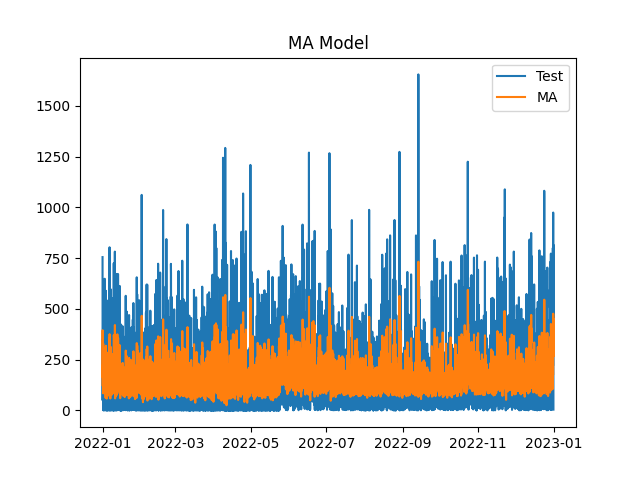
\includegraphics[width=0.8\textwidth]{plots/MA_model.png}
%     \caption{Previsões 2021 com modelo MA}
%     \label{fig:MA_model}
% \end{figure}
  
% \subsection{ARMA}

% AR eé blabla

% \begin{equation} \label{eq:ARMA}  y_t = \beta_0 + \beta_1 y_{t-1} + \dots + \beta_p y_{t-p} + \epsilon_t + \theta_1 \epsilon_{t-1} + \dots + \theta_q \epsilon_{t-q}  \end{equation}
% \textbf{ARMA (Autoregressive Moving Average) Model:}
% \begin{itemize}
%   \item{$y_t$: The value of the time series at time $t$.}
%   \item $p$: The number of time lags to regress on (AR part).
%   \item $q$: The number of time lags of the error term to regress on (MA part).
%   \item $\epsilon_t$: The error term at time $t$.
%   \item $\beta$: The coefficients of the lagged values (AR part).
%   \item $\theta$: The coefficients of the lagged error terms (MA part).
% \end{itemize}


% \begin{figure}[H]
%     \centering
%     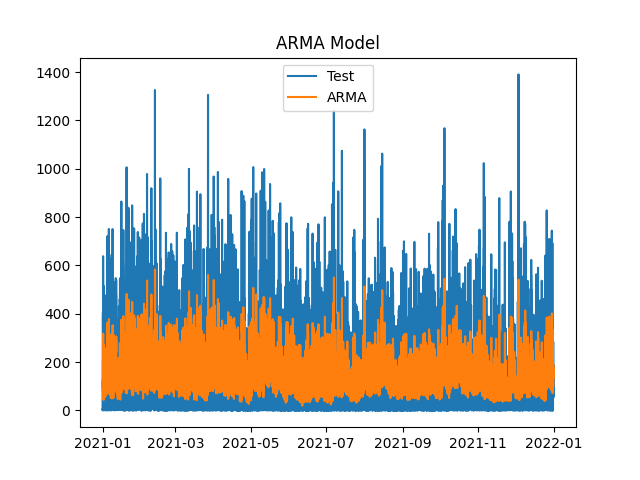
\includegraphics[width=0.8\textwidth]{plots/ARMA_model.png}
%     \caption{Previsões 2021 com modelo ARMA}
%     \label{fig:ARMA_model}
% \end{figure}

% \subsection{ARIMA}

% AR eé blabla

% \begin{equation} \label{eq:ARIMA}y_t^d = \beta_0 + \beta_1 y_{t-1}^d + \dots + \beta_p y_{t-p}^d + \epsilon_t^d + \theta_1 \epsilon_{t-1}^d + \dots + \theta_q \epsilon_{t-q}^d \end{equation}
% \textbf{ARIMA (Autoregressive Integrated Moving Average) Model:}
% \begin{itemize}
%   \item $y_t^{[d]}$: The differenced value of the time series at time $t$.
%   \item $p$: The number of time lags to regress on (AR part).
%   \item $d$: The order of differencing.
%   \item $q$: The number of time lags of the error term to regress on (MA part).
%   \item $\epsilon_t^{[d]}$: The differenced error term at time $t$.
%   \item $\beta$: The coefficients of the lagged values (AR part).
%   \item $\theta$: The coefficients of the lagged error terms (MA part).
% \end{itemize}

% \begin{figure}[H]
%     \centering
%     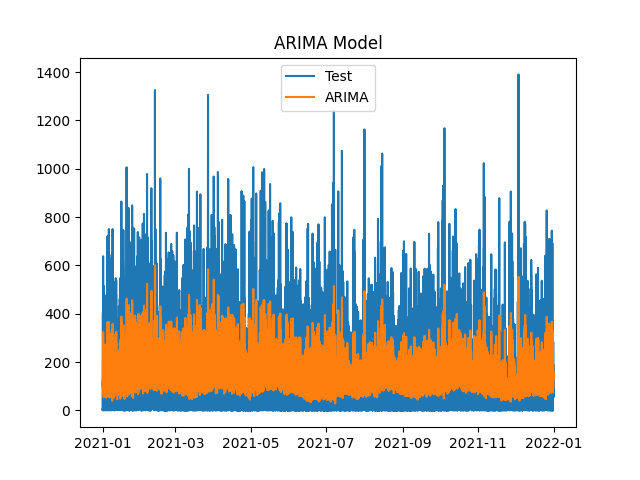
\includegraphics[width=0.8\textwidth]{plots/ARIMA_model.png}
%     \caption{Previsões 2021 com modelo ARIMA}
%     \label{fig:ARIMA_model}
% \end{figure}

% \subsection{SARIMA}

% AR eé blabla



% AR eé blabla

% \begin{equation} \label{eq:SARIMA} y_t^{[m]d} = \beta_0 + \beta_1 y_{t-m}^{[m]d} + \dots + \beta_p y_{t-pm}^{[m]d} + \epsilon_t^{[m]d} + \theta_1 \epsilon_{t-m}^{[m]d} + \dots + \theta_q \epsilon_{t-qm}^{[m]d} \end{equation}

% \textbf{SARIMA (Seasonal Autoregressive Integrated Moving Average) Model:}
% \begin{itemize}
%   \item $y_t^{[m]d}$: The differenced value of the time series at time $t$.
%   \item $p$: The number of time lags to regress on (AR part).
%   \item $d$: The order of differencing.
%   \item $q$: The number of time lags of the error term to regress on (MA part).
%   \item $m$: The number of time lags comprising one full period of seasonality.
%   \item $\epsilon_t^{[m]d}$: The differenced error term at time $t$.
%   \item $\beta$: The coefficients of the lagged values (AR part).
%   \item $\theta$: The coefficients of the lagged error terms (MA part).
% \end{itemize}

% \begin{figure}[H]
%     \centering
%     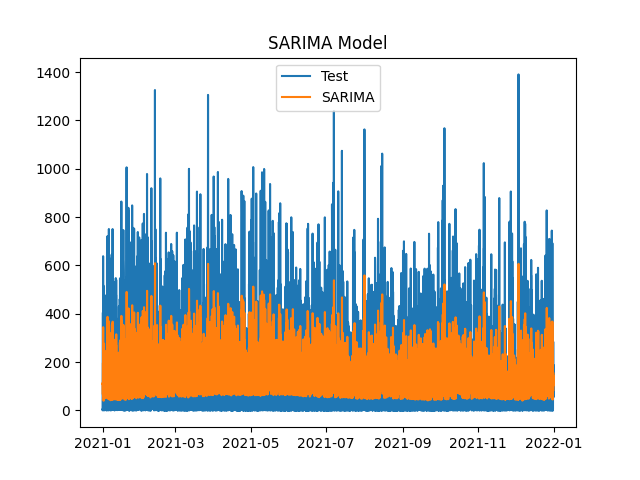
\includegraphics[width=0.8\textwidth]{plots/SARIMA_model.png}
%     \caption{Previsões 2021 com modelo SARIMA}
%     \label{fig:SARIMA_model}
% \end{figure}


% \begin{figure}[H]
%     \centering
%     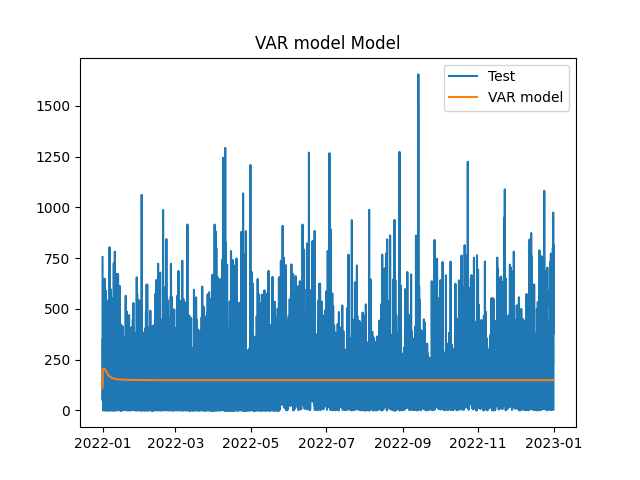
\includegraphics[width=0.8\textwidth]{plots/VAR model_model.png}
%     \caption{Previsões 2021 com modelo VAR}
%     \label{fig:VAR_model}
% \end{figure}









% \subsection{Resultados\label{se:statitics_scores}}

% \begin{table}[H]
%     \caption{Resultados modelos Estatísticos}
%     \resizebox{\linewidth}{!}{\begin{tabular}{llllllllll}
\toprule
rmse & abs erro & erro comp & r2 score & mape score & alloc missing & alloc surplus & optimal percentage & better allocation & beter percentage \\
\midrule
NaN & 0.00 & True & -0.65 & NaN & NaN & NaN & 0.00 & 0.00 & 0.00 \\
171.14 & 1123214.13 & True & 0.14 & 17.04 & 560507.02 & 562707.11 & 63.79 & 63.79 & 86.84 \\
169.99 & 1108555.94 & True & 0.15 & 16.36 & 554443.34 & 554112.60 & 64.04 & 64.04 & 87.17 \\
170.13 & 1111215.12 & True & 0.15 & 16.52 & 556281.62 & 554933.50 & 64.03 & 64.03 & 87.01 \\
171.88 & 1115725.36 & True & 0.13 & 16.43 & 568538.03 & 547187.33 & 63.45 & 63.45 & 86.92 \\
184.60 & 1253196.02 & True & -0.00 & 21.63 & 619929.79 & 633266.23 & 64.82 & 64.82 & 86.07 \\
\bottomrule
\end{tabular}
\label{tb:statitics_scores}}      
% \end{table}

% Apenas pelos métodos estatisticos verificamos que no ano de 2021 teria havido uma melhoria de cerca de 80\% das vezes, usando qualquer um dos métodos apresentados.\\
% Embora a alocação em falta seja de uma ordem de grandeza superior.\\


% \section{Treino e Resultados\label{se:training}}

% Realizaram-se várias experiências, onde em cada um se ia elimando alguns dos objectos em estudo.\\
% Em casa experiências toda a parametrização era igual, à excepção do objecto de estudo.\\

% \subsection{Arquiteturas e numeros de epocas}

% Nesta experiência foi testado o resultado das várias arquiteturas em estudo, como também o impacto do número de epocas na qualidade dos modelos.\\
% As arquitecturas estudadas foram:

% %TODO: arranjar reseach para cada uma 

% \begin{itemize}
%     \item[--] VanillaDense
%     \item[--] VanillaCNN
%     \item[--] VanillaLSTM
%     \item[--] StackedCNN
%     \item[--] StackedLSTM
%     \item[--] EncoderDecoder
%     \item[--] UNET
% \end{itemize}

% O modelos foram treinados em 200 epocas, sendo que foram salvos a cada 10 epocas, de forma conseguirmos perceber os contextos nos saltos de epocas.\\

% As parametrizações usadas:
% \begin{itemize}
%     \item[--] loss : mean squared error
%     \item[--] Metodo activação no meio : relu
%     \item[--] Metodo activação no fim : relu
%     \item[--] optimizador : Adam
%     \item[--] Janela temporal em X : 168 horas (1 semana)
%     \item[--] Janela temporal em Y : 24 horas (1 semana)
%     \item[--] Fracção de treino : 95\%  
% \end{itemize}

% \subsection{Funções de Perda (Loss)}

% TODO: o que é a loss function?

% Esta experiência consiste em rever que função de perda é melhor aplicavel ao problema. Sendo um problema de regressao linear, de valores bastante oscilatórios e com uma distribuição exponencial, temos algumas loss functions que já são reconhecidas para o problema.\\



% \begin{itemize}
%     \item[--] mean absolute error
%     \item[--] mean squared error    
%     \item[--] loss : mean absolute error

% \end{itemize}



% \subsection{Hiperparametrização}

% \subsubsection{Activação}

% \subsubsection{Optimizadores}

% \subsection{Janelas Temporais}

% Um dos pontos deste trabalho é perceber a fesiabilidade de usar dados de previsão do dia anterior (DA) para estes atributos energéticos.\\
% Algo que pode ser também aplicado no futuro a outros dados que não DA, mas sim a 3 horas, ou a 8 horas.\\
% Para perceber esta flexibilidade, mas especialmente para escolher as melhores janelas temporais a usar neste modelos, vamos testar várias combinações.\\
% Mantendo em mente que o objectivo é prever 24 horas, para os casos onde o alvo não dá um previsão de 24 horas, é necessario criar um número de modelos para fazer as 24 horas.\\
% Para validação apenas é usado o espaço temporar previsto, e não multiplos modelos.\\
% Dado as análises de autocorrelação iremos usar como janelas para treino o conjunto [24, 48, 98, 168] para prever o conjunto [1, 4, 8, 12, 24]\\
% Para alem destes foram também testadas combinações com janelas de treino 8 e 12 horas. Estas mostraram rapidamente que janelas de treino menores que as de previsão funcionam muito mal.\\

% \subsection{Classificação}

% Como descrito em (ref)... existe também o uso de tanto classes como valores linears para resolução de problemas de regressão, também chamado \textit{cluster-wise regression}.\\
% Para este teste mudamos um pouco o modelo em uso. Ao invés de apenas uma camada interpretativa, fazemos duas, em paralelo, sendo que uma resolve a regressão e a outra a classificação.\\
% Outro caso, proposto aqui, é usar uma nova camada interpretativa, que combina as duas saidas anteriores (linear e classificação), e resolve novamente para os valores lineares.\\
% Estes modelos não teram apenas uma saida, mas varias, como as arquiteturas MultiTail, mas neste caso cada uma resolve para um problema diferente, com funções de perda, e activações diferentes.\\

% TODO: desenho destas duas camadas intrepretaticas

% \subsection{Pesos}

% Por ultimo foi testado o impacto do uso de pesos nos modelos. Estes pesos são o peso que aquele alvo TODO: epxlicar pesos

% \subsubsection{Modelos lineares}

% Para os modelos lineares o peso que é adiciona ao modelo é a distância à média.\\
% Este peso serve para dar mais importância a valores facilmente considerados outliers.\\



% \subsubsection{Modelos Lineares e de Classificação}
% Aqui o peso é dado por saida. Para as saidas lineares o peso dados é o mesmo que apresentado anteriormente, para a saida de classificação, o peso é o inverso da frequência da classe.\\
% Distribuindo assim a importância de treino pela frquência das classes. Sendo um prática comum especialmente quando as distribuiçoes são muito desiguais, como o caso em estudo.\\
% É aqui estudada a aplicação destes pesos individualmente, e em conjunto. \\
% Os pesos aqui são também normalizados de modo a que o maior peso em cada um deles seja 1, e logo a multiplicação dos dois esteja dentro das mesmas dimensões de relevância.\\


% \begin{equation} \label{eq:peso_media} 
%     P_m = \left| y - mean \right| 
% \end{equation}

% \section{Considerações adicionais  \label{se:metodos_plus}}

% Foram realizados testes adicionais que não obtiveram resultados passivos de boa interpretação, e foram imediatamente descartados, como:

% \begin{itemize}
%     \item[--] Janela temporal em X : 96, 48, 24
%     \item[--] optimizador : todos os optimizadores disponiveis na biblioteca keras
%     \item[--] loss : todas as outra loss functions de regressão disponiveis.
%     \item[--] epocas : influência do número de epocas nos modelos, foram treinados até 20000 epocas alguns modelos mas à medida que a perda ia estagnando na assintomta, o modelo ia apenas piorando.
% \end{itemize}


% Todos os metodos foram realizados utilizando código em python, que está aberto em https://github.com/JotaFan/renewable-generation-into-reserve-markets
